% !TEX encoding = UTF-8 Unicode
% !TEX root =  ../Bachelorarbeit.tex

\chapter*{Exposé}
\label{cha:Expose}

\thispagestyle{empty}

Our cities have a problem! Our cities are built for cars not for humans. More and more people want to live next to places they want to reach and to commute less. Despite the desire for walkable cities our cities are slow to change. 
\\
To show what changes may be possible alternatives to the current state should be presented to inspire a new way to think about urban planning.  In order to present alternatives, this work will show how cities can be generated using procedural content generation (\FachbegriffSpezialA{PCG}{procedural content generation}{»short for procedural content generation. a method of creating data algorithmically, typically through a combination of human-generated content and algorithms coupled with computer-generated randomness and processing power.« \Zitat[see (1)]{Wikipedia:PCG}}{PCG}). PCG is a technique in which new universal patterns can be created from given patterns and rules. A prominent algorithm for PCG is wave function collapse (\FachbegriffSpezialA{WFC}{wave function collapse}{»short for wave function collapse. A special algorithm to solve problems by reducing a set of various states to a single state« \Zitat[see (2)]{Wikipedia:WFC}}{WFC}). WFC is a problem-solving algorithm that represents a possible solution as a set of solution elements in a superposition similar to quantum mechanics. These superpositions are broken down into a single state according to defined rules inside the algorithm.  WFC is a conventional algorithm that has been in use since 1978 \Zitat[Procedural Content Generation]{Wikipedia:PCG} Since then he WFC algorithm has been expanded to be used in different scenarios and for different purposes. In 2019 Kim Hwanhee et al. showed how to expand WFC to work on Graph based sets instead of only working on grids \Zitat[WFC on Graphs]{WFC:Graph-based}. This allows the Algorithm to work on 3 Dimensional systems as well. In 2022 Maxim Gumin et al. expanded WFC by using markov chains to create 3-dimensional buildings \Zitat [WFC using Markov Chains] {Github:MarkovJunior}. 
\\
\\

\begin{figure} [ht]
  \centering
  \includegraphics[trim={0 6.6cm 0 14cm},clip, width=1\textwidth]{Bilder/MaximGuminBuilding1.png}\
    \caption{\Zitat[Markov Chain Architecture]{Github:MarkovJunior}}
  \label{fig:gliederung}
\end{figure}

\section{Concept} 
This thesis discusses how to procedurally generate cities using wave function collapse considering factors like walkability, population density, and urban functionality. The thesis aims to explore realistic city constraints, generates building graphs with the previously mentioned constraints using WFC and finally renders 3d Models out of the building graphs. If there's enough time, it should be implemented to make the generation process parameter driven. Parameters could be walkability with a factor of 1 minute - 100 minutes, meaning that within the set time every individual should be able to reach their work, recreational facilities and grocery stores. Another interesting parameter could be population density. Ranging from  10-20.000 people per km². Or even ecological constraints like minimal amount of parks, greenery tiles, floodplains, balcony power plants, public transport vehicles, waste recycling facilities, agriculture and vertical farms, air-conditioned and heat save spaces and water use per population. In the 2023 publication \Zitat [Planning Climate Action in Cities and Regions]{City-planning:Climate-Actions} extensive measurements are listed that any city can take to minimize the effects of climate change.
\\
\\
Within this thesis the following steps will explained. 
\begin{enumerate}
    \item Research different buildings, their types, sizes, how much population they can support and what they need to function. A City consist of an uncountable amount of different buildings. Reducing and grouping them into easily understandable categories will help with writing the algorithm.
    \item Creating a foundation for the PCG algorithm by creating a \FachbegriffSpezialA{irregular quadrilateral grid}{}{»An object that contains only quads but resembles an organic shape«}{irregular quadrilateral grid}. Cities aren't build on square grids and using them as a basis would lead to many design flaws in later.
    \item Defining constraints for the different building types and how they should be implemented inside the algorithm. It must be researched which building has which real world constraint. For example how many people live in an apartment building or how many people can shop in a grocery store of size \(x\) and how many people can reach that store within a predetermined reach ability \(r\).  
    \item Writing the WFC algorithm that solves how buildings could be set up considering all given constraints. A proven method for this could be to iterate over the vertices of the previously created irregular quadrilateral grid and assigning each vertex a building class.
    \item For visualization a tile set has to be created 
    \item Finally a three dimensional model and an image should be rendered. With all the previously created information a \FachbegriffSpezialA{marching square algorithm}{}{»an algorithm that generates contours for a two-dimensional scalar field. \Zitat[Marching Squares]{Wikipedia:marching-squares}«}{marching square algorithm} can replace all tiles of the empty quadrilateral grid with tiles from the tile set
\end{enumerate}
The Tile set should be created in Blender using a simple low poly style inspired by Oskar Stålbergs Townscaper.
The code should be written in python which can be imported into blender using the scripting tab.

\begin{figure} [ht]
  \centering
  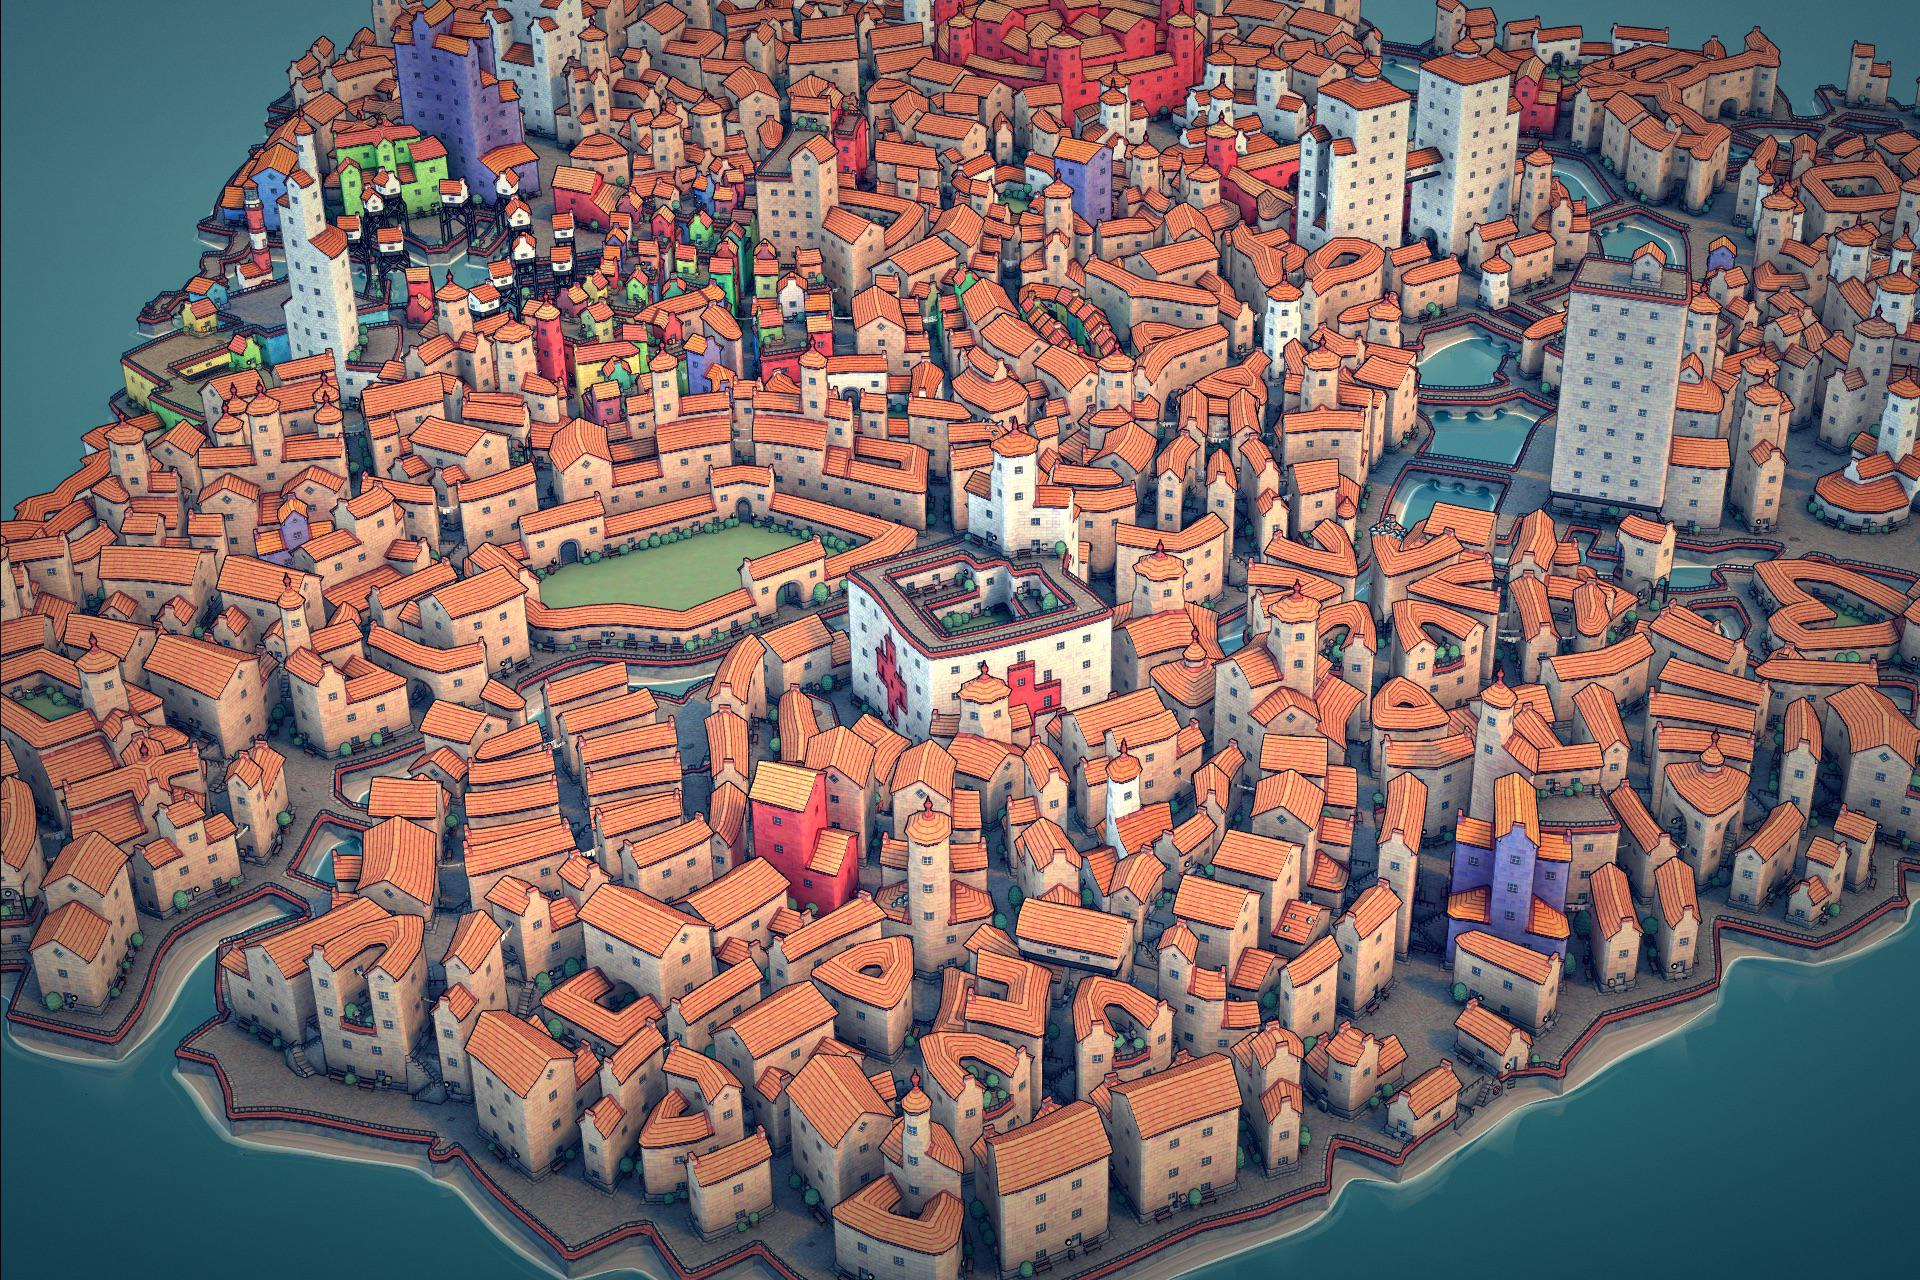
\includegraphics[width=0.4\textwidth]{Bilder/Townscaper.png}
    \caption{\Zitat[Townscaper]{Game:Townscaper}}
  \label{fig:gliederung}
\end{figure}

\section{Outline (not final)}
\begin{enumerate}
    \item Introduction
    \item City planning
    \begin{enumerate}
        \item Real world constraints
        \item Changes due to climate change impact on building metrics
        \item Walkability
        \item Constraint Database
    \end{enumerate}
    \item Procedural Content Generation
    \begin{enumerate}
        \item Wave Function Collapse
        \item Marching Squares
        \item Visualization
    \end{enumerate}
    \item Conclusion
\end{enumerate}

\section{Time schedule}
\begin{itemize}
    \item until 12.04 Anmeldung
    \item until 19.04 Research Buildings and Constraints
    \item until 03.05 WFC Algorithm ready (not visualization)
    \item until 17.05 Write Intro and City Planning part (rough version)
    \item until 31.05 Create Tile set and visualization
    \item until 14.06 Write PCG part and conclusion (rough version)
    \item until 05.07 revision and correction
    \item until 10.07 Print
    \item until 12.07 Abgabe 
\end{itemize}




